%==================================================================================================
% LaTeX paper template - use as a starting point for structuring a research paper.
%
% Written by Colin Perkins (https://csperkins.org/)
% 2002-2018
%
% To the extent possible under law, the author(s) have dedicated all copyright and
% related and neighbouring rights to this software to the public domain worldwide.
% This template is distributed without any warranty.
%
% You should have received a copy of the CC0 Public Domain Dedication along with
% this software. If not, see <http://creativecommons.org/publicdomain/zero/1.0/>.
%
% NOTE: The above Public Domain Dedication applies only to the LaTeX paper
% template distributed from https://github.com/csperkins/project-template
% in the file papers/example.tex. Unless explicitly stated, modifications 
% or additions to that template are copyright by their respective authors.
%==================================================================================================

%==================================================================================================
% General advice on technical writing:
%  - George Gopen and Judith Swan, "The Science of Scientific Writing",
%    American Scientist, Nov/Dec 1990. 
%    http://www.americanscientist.org/issues/num2/the-science-of-scientific-writing/1
%  - Stephen Pinker, "The Sense of Style: The Thinking Person's Guide to
%    Writing in the 21st Century", Penguin, Sept 2014. ISBN 0525427929.
%
% The paper writing advice in the comments is derived from talks and articles
% by Simon Peyton-Jones, Jim Kurose, Henning Schulzrinne, and Jim Bednar: 
%  - http://research.microsoft.com/~simonpj/papers/giving-a-talk/giving-a-talk.htm
%  - http://research.microsoft.com/~simonpj/papers/giving-a-talk/writing-a-paper-slides.pdf
%  - http://gaia.cs.umass.edu/kurose/talks/top_10_tips_for_writing_a_paper.ppt
%  - http://www-net.cs.umass.edu/kurose/writing/intro-style.html
%  - http://www.cs.columbia.edu/~hgs/etc/writing-style.html
%  - http://homepages.inf.ed.ac.uk/jbednar/writingtips.html
%  - http://www.gabbay.org.uk/blog/paper-writing.html
%  - http://homes.cs.washington.edu/~mernst/advice/write-technical-paper.html
%  - http://dx.doi.org/10.1371/journal.pcbi.1005619
%
% LaTeX usage notes:
%  - http://www.read.seas.harvard.edu/~kohler/latex.html
%
%==================================================================================================

%==================================================================================================
% The \documentclass{} macro specifies the overall style. For computer
% networking papers, common options are:
%
%   \documentclass[twocolumn,a4paper]{article}  % Base LaTeX style
%   \documentclass[conference]{IEEEtran}        % IEEE Conference
%   \documentclass[10pt,sigconf]{acmart}        % ACM SIGCOMM conference
%
% The IEEE and ACM templates are included in the lib/tex/inputs directory,
% but check for updates and use the version specified by the conference or
% journal to which you're submitting.

\documentclass[10pt,sigconf]{acmart}

% The following packages are recommended, and should be available in most
% standard LaTeX installations (or from https://www.ctan.org/). Note that 
% the order in which packages are loaded is significant.

% Basic extensions recommended for all LaTeX documents:
%   nag        Warn about common problems with LaTeX files
%   inputenc   Specify the character set used in .tex files
%   babel      Language-specific typography and hyphenation
%   microtype  Improved typography when generating PDF files

\usepackage[l2tabu,orthodox]{nag}
\usepackage[utf8x]{inputenc}
\usepackage[british]{babel}
\usepackage{ifpdf}
\ifpdf
  \usepackage{microtype}
\fi

% The AMS mathematics library greatly extends and improves mathematics
% support in LaTeX (see http://ctan.org/pkg/amsmath for details). When
%  preparing multi-line numbered equations, be sure to use:
%
%   \begin{align}
%     ...
%   \end{align} 
%
% rather than:
%
%   \begin{eqnarray}
%     ...
%   \end{eqnarray}.  
%
% when this package is loaded, to ensure they formatting is consistent
% (see https://tug.org/pracjourn/2006-4/madsen/madsen.pdf for details).

\usepackage{amsmath}
\usepackage[all]{onlyamsmath}

% Use Times, Helvetica, and Courier fonts, rather than Computer Modern:

\makeatletter
\@ifclassloaded{acmart}{
  % The ACM article style sets the fonts internally
}{
  \usepackage{newtxtext}
  \usepackage{newtxmath}
}
\makeatother

% Add support for sub-figures within a figure, as follows:
%
%   \begin{figure}
%     \centering
%     \subfloat[caption for 1st subfloat]{
%       \includegraphics{...}
%       \label{...}
%     }
%     \\
%     \subfloat[caption for 2nd subfloat]{
%       \includegraphics{...}
%       \label{...}
%     }
%     \caption{caption for entire figure}
%     \label{...}
%   \end{figure*}
%
% The subfig package obsoletes the older subfigure package, and is itself
% deprecated in favour of the subcaption package. However, as of April 2015
% subcaption doesn't work with ACM or IEEE style files (this is also the
% reason for the [caption=false] option).

\usepackage[caption=false]{subfig}

% Improve formatting of tables. To produce nice looking tables:
%
%   - avoid vertical lines;
%   - avoid double horizontal lines;
%   - use horizontal lines above and below the table, and to separate the
%     header from the body of the table, but not elsewhere; and
%   - if in doubt, align columns to the left (columns of numbers should
%     align to the decimal point)
%
% This translates to a tabular environment that looks something like the
% following:
%
%   \begin{tabular}{lll}
%     \toprule
%        Header1 & Header2 & Header3 \\
%     \midrule
%        Line1   & ...     & ...     \\
%        Line2   & ...     & ...     \\
%        Line3   & ...     & ...     \\
%        Line4   & ...     & ...     \\
%     \bottomrule
%   \end{tabular}

\usepackage{booktabs}

% Improve formatting for quote marks in verbatim mode:
\usepackage{upquote}

% Improve support for graphics:
\usepackage{graphicx}

% Add support for URLs using \url{...}. This formats the URL in typewriter
% font, and makes it a hyperlink if the hyperref package is also loaded.
\usepackage{url}

% Add support for drawing packet headers. For instructions, see
% http://ctan.org/tex-archive/macros/latex/contrib/bytefield
\usepackage{bytefield}

% Add support for typesetting program source code. You can either include
% code in-line:
%
%   \begin{lstlisting}[language=Python]
%   Source code goes here
%   \end{lstlisting}
%
% or include a source file:
%
%  \lstinputlisting[language=Python]{source_filename.py}
%
% This package is highly customisable and supports a range of languages.
% See package documentation at https://ctan.org/pkg/listings for details.
\usepackage{listings}

% Generated PDF files can include hyperlinks for URLs and cross-references
% using the hyperref package. This package, however, can interact poorly
% with others. Known issues include:
%
%  - Papers typeset without page numbers gives warnings of the form:
%      "pdfTeX warning (ext4): destination with the same identifier 
%      (name{page.}) has been already used, duplicate ignored".
%    since hyperref tries to refer to the page number.
%  - The algorithmic package uses the same line-numbering scheme for each
%    algorithm, and can cause duplicate identifier warnings if you have
%    several algorithms with line numbers (this may have been fixed with 
%    recent versions of algorithmic...).
%  - If using the algorithm package with hyperref, you need to load packages
%    in the following order (see README in hyperref documentation):
%      \usepackage{float}
%      \usepackage{hyperref}
%      \usepackage{algorithm}
% For these reasons, hyperref is best to avoid for most papers, however if
% needed, uncomment the following two lines:
%  \usepackage{float}
%  \usepackage{hyperref}

% The algorithm package defines the algorithm environment. This is used in
% the same way as the figure and table environments, to include algorithms
% in a paper. The algpseudocode package provides the ability to typeset the
% algorithms: http://ctan.org/tex-archive/macros/latex/contrib/algorithmicx
\usepackage{algorithm}
\usepackage{algpseudocode}
\usepackage{color}
\usepackage[bottom]{footmisc}

% By default, LaTeX adds extra space after punctuation. The \frenchspacing
% command disables this. This creates tighter looking, more even, text and
% avoids inconsistencies if you forget to use '\ ' to suppress the spacing
% after in-sentence punctuation.
\frenchspacing

% Prevent hyphenation of all upper case words:
\uchyph=0

% The ACM style needs \maketitle after the abstract, but the other styles
% want it before; these macros hide the difference and are used below:
\makeatletter
\@ifclassloaded{acmart}{
  \newcommand{\maketitleSTD}{}
  \newcommand{\maketitleACM}{\maketitle}
}{
  \newcommand{\maketitleSTD}{\maketitle}
  \newcommand{\maketitleACM}{}
}
\makeatother

% Define a simple \todo{...} macro:
\newcommand{\todo}[1]{\textbf{\textcolor{red}{To do: #1}}}

%==================================================================================================
\begin{document}
% Specify the title of the document:

\title{Year 1 PhD Progress Report}

% Specify the authors of the document. Unfortunately, there's no consistent
% way to do this that works across the different document classes. 
%
% If using \documentclass{article}:
%
%   \author{
%      A. N. Other\\University of Glasgow
%   \and
%      Colin Perkins\\University of Glasgow
%   }
%
% If using \documentclass{IEEEtran}:
%
%   \author{
%     \IEEEauthorblockN{A. N. Other}
%     \IEEEauthorblockA{University of Glasgow}
%   \and
%     \IEEEauthorblockN{Colin Perkins}
%     \IEEEauthorblockA{University of Glasgow}
%   }
%
% If using \documentclass{acmart} add a block like the following per author:
%
%   \author{Colin Perkins}
%   \orcid{0000-0002-3404-8964}
%   \affiliation{
%     \institution{University of Glasgow}
%     \streetaddress{School of Computing Science}
%     \city{Glasgow}
%     \postcode{G12 8QQ}
%     \country{UK}
%   }
%   \email{csp@csperkins.org}
%
% If you don't have an ORCID identifier, sign up for one at https://orcid.org

\author{Vivian Band}
\affiliation{
  \institution{University of Glasgow}
  \streetaddress{School of Computing Science}
  \city{Glasgow}
  \postcode{G12 8QQ}
  \country{UK}
}
\email{v.band.1@research.gla.ac.uk}

% Specify metadata about the paper. Again, what is required depends on the
% document class. If using \documentclass{acmart}, specify the following:
%
%   \acmYear{2018}
%   \copyrightyear{2018}
%   \setcopyright{acmcopyright}
%   \acmConference{CoNEXT '18}{December 4--7, 2018}{Heraklion/Crete, Greece}
%   \acmPrice{15.00}
%   \acmDOI{10.1145/3284850.3284856}
%   \acmISBN{978-1-4503-6082-1/18/12}
%
% The complete metadata is likely only available when preparing the final,
% camera ready, version of the paper.

\maketitleACM

%==================================================================================================
\section{Initial Reading}

% Literature survey
When I accepted the PhD offer, I took this as an opportunity to dedicate several years to studying a topic which has been of personal interest for some time: malware.
This was the starting point of my research readings during my first year, and this survey section will start with a review of the papers I read as part of my initial efforts to find a research angle on this topic.
My next step was trying to connect this recent reading about malware and online threats to areas I already have some experience of as a result of past research internships and level 4 and 5 research projects.
%I was already attempting to learn a new domain by reading malware and threat research articles, attempting to learn another unfamiliar domain in addition to this would have less chance of leading to a productive research topic than integrating my existing knowledge of network protocol design.
Sections \ref{malware-in-transit} reflects on the papers read during this stage.

A paper presentation I watched at a conference last year encouraged me to read into the wider context of cybercrime and to consider moving my research beyond solely technical analysis.
This is discussed in section \ref{cybersecurity}.

A pattern that I noticed being repeated in several network measurement papers was the use of scans of the IPv4 address space.
This led me to read about strategies to scan the IPv6 address space, and to the realisation that IPv6 address space scanning is difficult to perform even for benign purposes like local network maintenance;
its use for host recruitment by malicious actors remains an open research question.
My readings into network scanning methods and IPv6 scanning strategies are discussed in section \ref{internet-scanning}.


\subsection{Malware Samples}
\label{malware-reading}
Several of the first papers I found when searching for malware and security research topics were heavily platform- or language-dependent, like surveys of Android platform security \cite{bhat2019} \cite{tam2017}, writing a kernel in Rust \cite{levy2017}, or preventing code reuse attacks in C++ \cite{schuster2015}.
These were interesting reads, but it was recommended that I direct my search towards more general topics, which were not focused on a specific technology.
This led to reading papers which could be used to improve the process of analysing malicious binaries, for combinations of both static and dynamic analysis \cite{or-meir2017} \cite{afianian2019} \cite{izumida2010} \cite{izumida2018} \cite{mori2006}.
\footnote{Tomonori Izumida, the primary or co-author of \cite{mori2006}, \cite{izumida2010} and \cite{izumida2018}, is a researcher at Internet Initiative Japan Innovation Institute (IIJ-II). I will be an intern at this location sometime in 2021, and hope to discuss this work with him while I am there.}
Malware authors use a range of obfuscation techniques, like binary packing and opaque constants, and there is a lot of ongoing research to adapt existing analysis tools to detect these techniques, or to use machine learning to recognise more ambiguous social engineering-based attacks \cite{maiorca2019}.


\subsection{Malware in Transit}
\label{malware-in-transit}
An alternate direction for the initial literature review was to look at potential research angles involving malicious traffic, given my past experience of working with network protocol development in the IETF and modifying both kernel and userspace network stacks.

Work by Costa et al. in 2005 proposed using network-level approaches for the automated containment of worms, a rapid, self-propagating class of malware \cite{costa2005}.
Their proposed system, Vigilante, allows hosts to share information about vulnerabilities in the form of machine-verifiable self-certified alerts (SCA).
These alerts are generated through the inspection of incoming network traffic, and distributed in a peer-to-peer manner to provide resilience against denial of service attacks and to avoid trusting a central server which could potentially by compromised.
While Vigilante is useful for detecting network payloads which can be decrypted at kernel-level or by another application at userspace level, it will likely fail on attempting to inspect traffic which is encrypted by a malicious application;
this is increasingly likely to be the case in the modern Internet, where encrypted payloads are now the default.
Work by Mori et al. on host-based detection in 2006 notes that even 14 years ago, malware was using self-encryption and polymorphic approaches to evade pattern-matching detection methods used by anti-virus software at the time \cite{mori2006};
polymorphism is still very common, with many modern ransomware variants compiling themselves on each install to produce custom ransom notes and with open-source malware like Mirai being adapted to greater or lesser degrees by many different authors.
Instead, they opt to detect worm-like programs by performing automated static analysis, then allowing the program to run in a simulator which allows the potential malware to perform calls to stub replacements for standard kernal API functions.
Adapting deep traffic inspection and suspicious API calls for a heavily encrypted userspace transport protocol like QUICcould prove to be an interesting future research question, and this was considered as an initial research topic.
However, this was still at an early stage of the initial literature review, and was similar to the Direct Code Execution \cite{tazaki2013} project I was supposed be doing at Internet Initiative Japan Innovation Institute (IIJ-II) last month (postponed until after the pandemic);
I decided to spend more time reading to see what other potential research topics were of interest.

\subsection{Cybercrime and Security}
\label{cybersecurity}
In October 2019 I attended the Internet Measurement Conference (IMC'19).
One of the talks focused a paper on the effects of police interventions on operators and clients of denial of service-for-hire services, known as `booters' \cite{collier2019}.
One particular finding was genuinely surprising:
simple web banner advertisements warning that booter services are illegal dissuades many potential new clients from using these services, and were even more effective at dissuasion than the arrests of the operators of these services.

I had a chance to talk with two of the authors of this paper, Ben Collier and Daniel Thomas, who are based at the University of Cambridge and the University of Strathclyde respectively.
This discussion was productive:
I learnt that my work did not have to be exclusively technical, and that I could take time to learn how to produce work with more of a social sciences angle if I felt the research topic required it.
This has been a key influence in the direction I want my PhD project to take;
the technical side of exploits and vulnerabilities is interesting, but understanding the social and economic influences behind the markets for malicious software is key to evaluating how likely it is that these exploits might actually be used in practice.

Research in this area is challenging, with many legal and ethical considerations to be aware of.
Another paper by Thomas et al. \cite{thomas2017} addresses issues with using `datasets of illicit origin', such as unauthorised data leaks, or unintentional data disclosure through user error.
The assertion in this paper is that all work completely or partially produced using datasets in this category should have an ethics section, discussing any potential harm which could have been caused to individuals in these datasets and the measures taken to minimise such harm.
I will need to carefully consider the ethical considerations of my PhD work;
many experiments can be conducted in controlled environments, but some, such as Internet-wide vulnerability scans, will need to be severely restricted or left entirely theoretical to avoid causing unnecessary harm.

\subsection{IPv6 Scanning}
\label{ipv6-reading}
While reading about an Internet-wide scan being performed for the entire 32-bit IPv4 address space by a botnet \cite{dainotte2014}, two questions occurred to me:
how would a scan of the 128-bit IPv6 space be performed, and how could a botnet recruit enough hosts in an IPv6-only environment to be viable?

Work by Murdock et al. \cite{murdock2017} describes tools which appear to use statistical modelling to generate lists of active IPv6 addresses in the wider Internet.
A paper by Gasser et al. \cite{gasser2016} explores a hybrid approach to building IPv6 hitlists, using both passive sampling of incoming traffic and active scanning;
as discussed in \cite{thomas2017}, this paper contains an ethics discussion reflecting on how active scans can be interpreted as malicious and can cause issues for hosts receiving active scanning traffic.
The dataset used for passive sampling in this study is from a large European Internet Exchange Point (IXP).
This is unlikely to be an accessible source of data for most attackers, but data obtained from publicly accessible DNS records and traceroutes could feasibly used to generate .

An article from a 2006 issue of `;login:', the Usenix magazine, details the specific scenario of how worms could spread through IPv6 networks \cite{bellovin2006}.
As one would expect of an article from 14 years ago, some of this information is outdated:
there is no mention of privacy addresses, a feature outlined in RFC 4941 \cite{rfc-privacy-ext} and used for IPv6 addressing in all modern, mainstream operating systems,
and the authors state that an ``informal poll'' of network operators suggests that servers would be addressed statically, towards the low end of the subnet address range;
IPv6 addresses are likely to be given to servers via dynamic host configuration protocol for IPv6 (DHCPv6).
However, the majority of the suggested sources of information still apply, such as gaining prefix information from Border Gateway Protocol (BGP) advertisements.
Some sources of address information may no longer apply to desktop and laptop devices which were in use in 2006, but have become relevant once again through the increasing popularity of poorly secured IoT devices:
media access control (MAC) addresses of IoT devices are unlikely to be obscured in an assigned IPv6 address by privacy extensions, so this can be used for reconnaisance by an attacker.
RFC 7707 \cite{rfc-ipv6-rec}, produced 10 years later in 2016, takes a far more in-depth technical view of IPv6 reconnaisance techniques, and provides a wealth of information about which patterns can be used to reduce the potential IPv6 search space down to a manageable range.
A particularly interesting detail in this document is that stateless address autoconfiguration (SLAAC) support is (in an ideal, RFC-compliant world) mandatory;
this potentially means that operating systems which use privacy extensions for IPv6 addressing could also allocate an address which exposes the interface's MAC address, possibly in addition to this obscured address.
RFC 7707, and this Usenix article, are both valuable starting points for learning how attackers might exploit information in IPv6 addresses for the discovery potentially vulnerable devices, potentially for use in botnets.


\subsection{Current reading}

Understanding the technical feasibility of malware using IPv6 for host recruitment is important;
this is obvious, and so I will continue reading more Internet standards documents and academic papers related to routing, security, and address space search algorithms in IPv6 networks.
However, understanding the context of modern cybercrime activities and economic trends in the malware `industry' is vital for evaluating how likely it is that any of the proposed attacks would be used, and which factors might affect this.
Making additional contacts and potentially collaborating with economics, sociology, and criminology researchers would be ideal for producing high quality work related to this area, as was the case with the booters paper by Collier et al. \cite{collier2019};
I have some knowledge of the technical details involved in attacks, but I am not yet qualified to carry out the social or economic science elements of these experiments.

Although the topic I have chosen, use of IPv6 scanning for host recruitment in malware, can be researched without any practical knowledge of malware analysis, learning this skill is key to understanding write-ups detailing current malware behaviours seen in the wild.
Knowing how to analyse malware samples, learning common compiler conventions, and understanding the quirks of different types of assembly code are all important for a career in industry research in this area.
To the best of my knowledge, malware using IPv6 scanning for host recruitment does not yet exist, but this could change over the next three years;
being able to perform first-hand analysis on such a sample would provide excellent material for a write-up or future publication.
I have taken the first steps towards fixing this gap in my knowledge by working through `The IDA Pro Book' \cite{ida-book}, Malware Unicorn online reverse engineering tutorials \cite{malware-unicorn}, and the textbook `Practical Malware Analysis' \cite{malware-analysis}, and will continue to develop these skills throughout the PhD.



%==================================================================================================
\section{Research Topic Background}

Malware and threat research is a fast-moving environment.
The core idea of researching the use of IPv6 scanning by malicious groups came from reading academic research papers, but much of the information about the business operations of cybercrime groups and malware authors is presented through blog posts and reports published by individuals and cybersecurity companies.
This section is therefore backed by citations from a combination of both academic sources, and from primary self-published resources from the information security community.

\subsection{Malware Lifecycles}

As more and more and more of their customers gained access to the Internet, many businesses made their services more convenient by moving them online.
The use of online services has become increasingly normalised in the decades since this initial move;
smartphone app use is pervasive in many countries, online shopping giants like Amazon have changed the commercial landscape, and entertainment services such as Netflix or online multiplayer gaming are commonplace.
The convenience offered by these services is clearly of high value to many people, and the rise in Internet-connected peripheral devices, known as the Internet of Things (IoT), is an extension of this:
`smart assistants' like the Amazon Alexa are explicitly marketed at non-technical users as a quality of life improvement, motion-activated cameras like Ring are sold as home privacy enhancements, and smart TVs are advertised as an easy way to enjoy streaming services in domestic settings.

Unfortunately, criminal organisations have also found a range of opportunities in these developments.
Millions of users submitting sensitive data, such as addresses and banking details, is a goldmine of information to malicious actors, who can easily use information held on a compromised server for identity theft or illicit financial gain.
Ransomware in particular has been on the rise in recent years, directly extorting payment from victims on the basis that that many businesses and individuals do not reliably back up important data.
Certain botnet variants, such as Mirai, IoT Reaper, and Mozi, focus specifically on recruiting poorly secured IoT devices left with default login credentials to launch Distributed Denial of Service (DDoS) attacks on key Internet infrastructe, such as DNS servers and Internet Service Providers \cite{antonakakris2017}.

The economy surrounding different types of malware has become increasingly complex as the range of devices on the market and associated attacks has increased.
Pay-Per-Install (PPI) services were common means of malware distribution in the early 2010s \cite{ppi};
clients (often, but not exclusively, malware authors) would approach a service to install their software on a number of machines in exchange for a fee.
The actors who would actually install these programs, known as affiliates, would earn commission based on how many instances of these programs they managed to install;
this was somewhat competitive, as affiliates developed exploits independently and had installs verified through the use of a unique code reported back to the PPI service.
PPI services have been superceded by Malware-as-a-Service (MaaS) operators, who typically deploy malware variants known as `loaders'.
These are designed to be subtle and persistent in order to act as a gateway for loading other malware onto infected systems;
other malware operators, typically ransomware gangs, rent these devices for a period of time to run their malware campaigns in exchange for a fixed fee or a cut of the profits \cite{emotet-lease}.

Loader malware typically enters machines through spam email campaigns, where a user attempts to open an email attachment of some sort or clicks a malicious link \cite{emotet-malspam} \cite{jasperloader}.
The malware can then spread laterally, infecting other hosts on the local network through IPv4 address space scans \ref{email-vector}.

\begin{figure}
\centering
        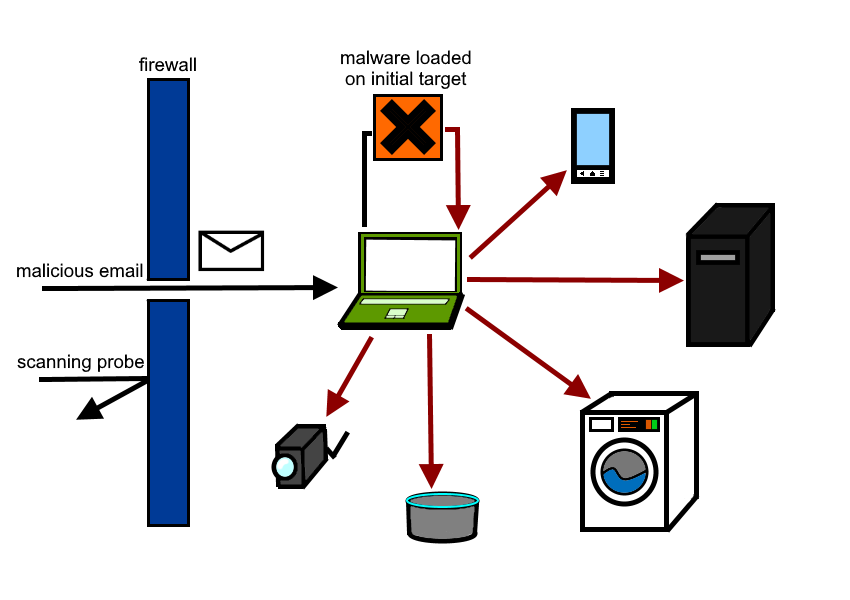
\includegraphics[totalheight=8cm]{email.png}
    \caption{A laptop becomes the initial infection vector on a local network. The malware gains access to the laptop through opening a malicious attachment or link; the firewall does not protect against this, since incoming email and web traffic are both allowed. Scanning probes, however, are blocked; no ports have been opened for IoT devices on this network, either manually or through UPnP.}
    \label{email-vector}
\end{figure}

The use of spam email campaigns with malicious payloads generally targets mainstream operating systems running on complex devices like smartphones, laptops, and desktops: devices with a graphical display and text inputs are common targets for keylogger software or popular ransomware variants.
However, this vector is not limited to these more complex devices: an ambitious criminal enterprise could also use lateral spread to install adapted loader software or otherwise compromise IoT devices on the same local network.
IoT devices are generally lightweight, and run their own custom operating systems to allow them to perform their required functions within certain constraints (eg. physical size, battery life);
security is often poorly implemented within these custom operating systems, and users often leave the default login credentials in place and fail to apply updates, making IoT devices easy targets for compromise.
Malicious spam campaigns targeting personal email accounts, rather than work accounts, are increasingly likely to gain entry to a network containing these poorly secured IoT devices which could capture unusual types of sensitive information:
a keylogger on a laptop or a smartphone can give information about banking details, passwords, and instant messages, but the compromise of an IoT device could lead to an attacker having access to anything from live audio and video feeds, to control of a home thermostat, to being able to start a fire in the victim's home \cite{candletouch}.

Initial compromise through email attachments is useful for host recruitment in cases where the host is adequately protected by a firewall from Internet-wide scans, for both IoT and for more complex devices:
a device such as a smartphone, laptop, or desktop acts as the initial vector, which goes on to infect other devices on the network.
However, many IoT devices intentionally weaken firewall security using a feature known as Universal Plug and Play (UPnP).
This automatically enables port forwarding on routers to enable access to IoT devices remotely, allowing users to access functionality like remote video feeds and thermostat adjustment while they are away from home.
While convienient for the user, this also allows attackers access to these devices;
in the case of Mirai malware variants, these exposed IoT devices are often recruited as part of a botnet used to launch DDoS attacks \cite{mirai-traffic}.

\begin{figure}
\centering
        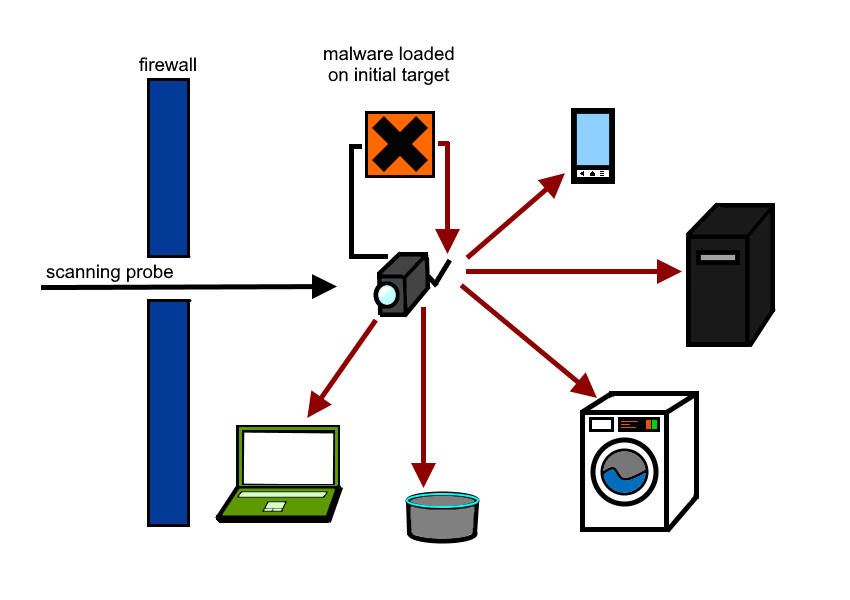
\includegraphics[totalheight=8cm]{scanning.png}
    \caption{A smart camera becomes the initial infection vector for devices on a home network. The device automatically allows traffic to bypass the firewall due to automatic port forwarding enabled by UPnP, allowing access to authorised and unauthorised users alike.}
    \label{iot-vector}
\end{figure}

IoT devices which do not require remote access, and complex devices which do not use UPnP, like smartphones and laptops, are generally not vulnerable to Internet-wide scans and would be more likely to become targets through lateral spread through local networks, as described earlier.
It is worth noting, however, that a UPnP-enabled IoT device recruited through the use of an Internet-wide scan could become the initial vector which compromises other devices on the local network, as shown in figure \ref{iot-vector};
this is effectively an inverse infection pattern to the malicious email scenario described earlier in figure \ref{email-vector}.


Both Internet-wide and local network scans continue to rely on scans of the IPv4 address space;
neither vectors have yet been adapted for use with IPv6.
UPnP is necessary in IPv4 networks due to network address translation (NAT), which was used to create the illusion of a larger IPv4 address space.
An attacker can gain access to an IoT device on a NAT-obscured network by performing a port scan against the IPv4 address assigned to the router, and is then free to compromise the device using the relevant exploit.
IPv6 solves the address shortage problem by creating a much larger address space for devices and therefore removes the need for UPnP;
end-to-end connectivity granted by IPv6 also allows any device to be directly routed to, not just machines with manually enabled port-forwarding or UPnP IoT devices as is currently the case.
It is believed that this larger address space improves security due to being too large to exhaustively scan.
This is not necessarily true:
the search space can be reduced to feasible ranges, and metadata embedded in IPv6 addresses, particularly in poorly secured IoT devices, can provide attackers with key information about devices which is not revealed by equivalent IPv4-based scans.

%==================================================================================================
\subsection{IPv6 Scanning for Malware-as-a-Service}

Recruitment of more devices is of interest to MaaS groups, given that an increased number of loader-infected devices increases their profits.
A combination of Internet-wide scans and local network scans for lateral spread will produce the highest yield of hosts;
IoT devices recruited through Internet-wide scans and devices infected by malicious email attachments or downloads can both serve as initial vectors, and both of these will make use of local network scans to detect and possibly compromise other hosts.
%Infected IoT devices are typically used to mount DDoS attacks, but could also be used to access sensitive information like live audio and video capture, or serve as initial entrance points for the lateral spread of loader malware across the local networks they belong to.
%They can also be used in ransomware campaigns, with users unable to gain access to an infected IoT device until the ransom is paid.
Internet-exposed IoT devices may even be a preferred route of compromise:
a user who may not fall for opening a suspicious email attachment may still have their other devices infected by a compromised IoT device without being aware an attack is even taking place.
Complex devices can become hosts to many different kinds of malware, but the wide range of purposes served by IoT devices also means that there is a potential market for leasing them for additional purposes in addition to typical Mirai-style DDoS attacks, such as accessing live audio or video capture, changing the displays of digital billboards, or holding key home infrastructure like smart thermostats to ransom.
As the number of purposes served by IoT devices grows, so does the range of potential use-cases for criminal enterprises  \cite{antonakakis2017}.


Both lateral spread through networks and mass recruitment through Internet-wide scans both currently rely on scans of the 32-bit IPv4 address space.
An exhaustive scan of the IPv4 address space on the wider Internet is trivial:
these can be performed in 5 minutes at a minimum, but are typically performed over a few hours to reduce suspicion.
As a result of widespread use of UPnP, these scans are capable of yielding thousands of hosts, with Mirai hosts generating over 1Tbps of DDoS traffic in an attack against DNS provider Dyn in 2016 \cite{mirai-traffic}.
An IPv4 scan on a local network is even easier, given that the search space is reduced further by a local netmask.

IPv6 addresses are 128 bits long, and are usually split into two 64-bit halves: the network prefix and the interface identifier.
An exhaustive search of this space is not feasible.
However, it can be reduced through publicly accessible information such as BGP advertisements and device metadata embedded in IPv6 addresses.
All modern operating systems for smartphones, laptops, and desktops obscure this information through the use of IPv6 privacy extensions, but the custom operating systems on IoT devices either openly expose this information, or obscure it poorly through weak random number generation.
This lack of obfuscation, combined with a general lack of focus on security, continues to make IoT devices an easy target for malicious actors, particularly when they can use this exposed metadata to determine which type of device has been infected and can therefore offer a more bespoke MaaS operation to potential clients;
this is not possible from address alone in IPv4 scans.
This also allows MaaS operators to conduct more focused scans, only targeting specific classes of devices while avoiding contact with devices which are not of interest in a particular campaign.
This minimises the amount of suspicious traffic generated by such scans, in contrast to IPv4 scans which are noisy and probe every reachable device on the network.

IPv4 addressing is unlikely to completely disappear in the next few decades, and malicious actors will continue to perform scans of this address space for mass host recruitment and for lateral spread of malware across local networks.
However, there is a persistent myth that switching to IPv6 is more secure because the address space is too large to exhaustively scan, and potentially an idea which could be taken as a quick security fix by IoT device manufacturers;
even if an IoT device only uses IPv6, it is still vulnerable to port scanning attacks if it does not employ robust IPv6 privacy addressing methods.

IoT devices are the primary focus of this PhD project due to the complete lack of privacy addressing in many instances, but, as described earlier, more complex devices like smartphones, laptops, and desktops are not immune from being compromised as a result of IPv6 scans.
According to RFC7707 \cite{rfc-ipv6-rec}, stateless address SLAAC support is mandatory for IPv6 address allocation;
this is the addressing method which leaves the MAC address of a device's network interface card (NIC) exposed in an allocated address.
More complex operating systems assign an IPv6 privacy address, which obscures the MAC address of the interface and therefore gives away less information about the device in outgoing traffic;
it is not clear if these are allocated in addition to these SLAAC addresses or as a replacement.
If they are an alternative rather than a replacement, then they only offer protection against passive eavesdropping of network traffic, and no resistance against active probing attacks.
This would expand the range of targets potentially generated by IPv6 scans for a determined attacker, and is therefore an important future point of investigation in this project.




%==================================================================================================
\section{Description of Current Work}

% Description of what's been done this year in terms of experiments/data

A good foundation for the rest of the PhD is proving that it is actually possible for attackers to exploit exposed information in IPv6 addresses.
An IPv6 address scanner does not need to scan the entire address space in order to be a plausible attack vector, it only needs to iterate through enough valid address ranges to yield a significant number of active targets in a feasible amount of time.
It also should to be possible to construct the scanner from publicly available information; 
attackers may be able to access valid IPv6 addresses illictly through other means, but would likely opt for methods which keep them as anonymous as possible as well as granting them a unique dataset for an economic advantage over similar groups.

\subsection{Local Host Scanning}
Lateral movement over local networks was the first scenario considered in the construction of an IPv6 scanner.
The first machine is infected with malware as a result of a user opening a malicious attachment and running a suspect file;
being able to inspect this first host gives the malicious application a wealth of information, including the 64-bit network prefix used in IPv6 addresses in this particular network.
This halves the search space, leaving the remaining 64 bits which make up the interface identifier.

The first half of a MAC address (ie. the first 24 bits) is known as an organisationally unique identifier (OUI), which is specific to the manufacturer of a given network interface card \cite{oui-list};
the second half of the address is specific to that card.
In SLAAC-assigned IPv6 addresses, this OUI is used as the first 24 bits in the network interface identifier half of the address.
The constant \texttt{0xFFFE} is used in the following 16 bits of the IPv6 address.
Given this information, we can state that the final search space for vulnerable IoT devices with SLAAC-assigned IPv6 addresses on a local network is n\*2\^24, where n is the number of OUIs being searched.
As stated previously, the IPv4 address space, with 2\^32 possible addresses, can be scanned in 5 minutes;
the address space for 256 different OUIs can be scanned in this time, making this a viable attack vector for finding a wide variety of IoT devices on a local network.

\subsection{Internet-Wide Host Scanning}
Malicious actors are keen to recruit hosts as widely as possible, particularly botnet operators and outfits who lease hosts to other malware operators;
a larger number of located targets translates into a business advantage for such parties, so an automated method of boosting these numbers as much as possible is an attractive prospect.
It is therefore important to consider the use-case of attackers performing Internet-wide scans of the IPv6 address space to find targets not adequately protected by firewalls.

BGP is used to exchange routing and reachability information between autonomous systems on the wider Internet.
BGPStream is an application which can be used to process historic BGP data gathered by points known as collectors \cite{bgpstream}.
Announcement messages are of particular interest to this scanning project:
these indicate that a new IPv6 network prefix was being advertised by an autonomous system, and shows an IPv6 network prefix which was in use at the time.
Each prefix is accompanied by a mask, which indicates how many bits must be set to specific values for that address;
as expected from the word `prefix', these bits are always set contiguously from the start of the address.
This is an integer usually between 29 and 64.

These announcement messages can be scraped using the BGPStream API to give a list of prefixes which were active on a given date and time.
Further filtering can be done on this list to remove any duplicate prefixes (ie. prefixes which were announced more than once), and to identify which prefixes are subsets of other prefixes
(ie. if two prefixes have the same address but different masks, the advertised prefix with the larger number as its mask is a subset of the prefix which has the smaller number, due to having more bits set to pre-determined values).

The tutorial for prefix monitoring on the BGPStream website \cite{bgpstream-tutorial} scrapes BGP data obtained over 5 hours on August 12th 2014.
This dataset was relatively small, and therefore a useful starting point for testing the scripts which removed duplicate address announcements and counted the number of instances of each prefix mask.
This process was repeated for gathering and processing IPv6 prefix announcement data over 5 hours on May 26th 2020, by the same collector which, theoretically, had the same view of the Internet as it did in 2014;
the 2020 dataset was much larger, containing 88,139 unique advertised prefixes, compared to the 2014 set which only had 1150.

\begin{table}[]
\centering
\label{ipv6-scanning}
\begin{center}
	\begin{tabular}{|l|l|l|}
		\hline
		IPv6 Prefix length & 2014 instances & 2020 instances   \\ \hline
		/16 & 0 & 1   \\ \hline
		/19 & 0 & 1   \\ \hline
		/20 & 0 & 13   \\ \hline
		/21 & 0 & 6  \\ \hline
		/22 & 0 & 7   \\ \hline
		/23 & 0 & 5   \\ \hline
		/24 & 2 & 26   \\ \hline
		/25 & 0 & 6   \\ \hline
		/26 & 0 & 14   \\ \hlinie
		/27 & 1 & 19   \\ \hline
		/28 & 4 & 106   \\ \hline
		/29 & 35 & 3049   \\ \hline
		/30 & 1 & 497   \\ \hline
		/31 & 0 & 206   \\ \hline
		/32 & 320 & 14399   \\ \hline
		/33 & 7 & 1673   \\ \hline
		/34 & 3 & 1374   \\ \hline
		/35 & 10 & 707   \\ \hline
		/36 & 56 & 3803   \\ \hline
		/37 & 0 & 599   \\ \hline
		/38 & 10 & 1061   \\ \hline
		/39 & 2 & 356   \\ \hline
		/40 & 62 & 4741   \\ \hline
		/41 & 1 & 591   \\ \hline
		/42 & 1 & 1103   \\ \hline
		/43 & 0 & 237   \\ \hline
		/44 & 69 & 5413   \\ \hline
		/45 & 5 & 603   \\ \hline
		/46 & 24 & 2296  \\ \hline
		/47 & 11 & 1457   \\ \hline
		/48 & 504 & 43205   \\ \hline
		/49 & 0 & 28   \\ \hline
		/50 & 0 & 2   \\ \hline
		/51 & 0 & 1   \\ \hline
		/52 & 3 & 12   \\ \hline
		/56 & 3 & 63   \\ \hline
		/59 & 0 & 3   \\ \hline
		/60 & 0 & 4   \\ \hline
		/62 & 0 & 1   \\ \hline
		/63 & 0 & 2   \\ \hline
		/64 & 13 & 397   \\ \hline
		/126 & 2 & 29   \\ \hline
		/128 & 1 & 20   \\ \hline
		/Total & 1150 & 88139   \\ \hline
		\hline
	\end{tabular}
	\caption{Number of instances of each prefix found over 5 hours of BGP IPv6 advertisements}
\end{center}
\end{table}


Although the raw number of prefixes have markedly increased, /48 prefixes remain the most frequently announced in both datasets:
43.8\% (504 announcements) in the 2014 set and 49.0\% (43205 announcements) in the 2020 set.
This means that 48 bits of the network prefix are already known.
Combined with the earlier knowledge that only 24 bits are unknown in the interface identifier half of an IPv6 address for a device with a SLAAC-assigned address, this gives a total search space of 40 bits for prefix announcements with a /48 mask.
An attacker could iterate through all possible combinations of these 40 bits, however, they do not have to search the space exhaustively;
any network prefix which consistently returns request timeouts is likely to be firewalled or not in use.
These prefixes can be discounted from the search, and the scanner can move onto searching the next possible prefix.
As such, it may be more helpful to think of the network prefix search space as somewhat independent of the interface identifier search space:
if, after a small number of ping attempts to different possible hosts (eg.100) on the same IPv6 network, the scanner does not receive a reply or a \texttt{Destination host unreachable} response, the prefix can be assumed to be unproductive and not worth searching further.
This means that /48 prefixes effectively have a search space of 16 bits, in order to iterate through all full 64-bit IPv6 network prefixes;
a collection of active prefixes can be found in under a minute, assuming a relatively small number of attempts are made to ping different hosts on all possible iterations of these 16 bits.
Any `live' prefixes which were found during this search can then be fully scanned for the remaining unknown 24 bits in the interface identifier.

/32 announcements were the second most common announced, making up 27.8\% of the 2014 set and 16.3\% of the 2020 set.
Announced prefixes with a mask smaller than 32 bits were rare:
3.6\% in 2014 and 4.7\% in 2020.
Given that 32-bit searches are possible in around 5 minutes, and that the network prefix and interface identifier search spaces are largely independent of each other, there are a very wide range of IPv6 network prefix ranges which can be searched in a feasible amount of time:
a single /32 advertisement could be searched exhaustively for valid network prefixes in around 5 minutes if only attempting one possible interface identifier, but would take n\*5 minutes when discarding inactive prefix configurations after n attempts, as described previously.
This is still feasible, but not as likely to produce results as quickly as searching through /48 advertisements.
/48 advertisements are therefore likely to remain a more popular target for these kinds of attacks.


\begin{figure}
\centering
        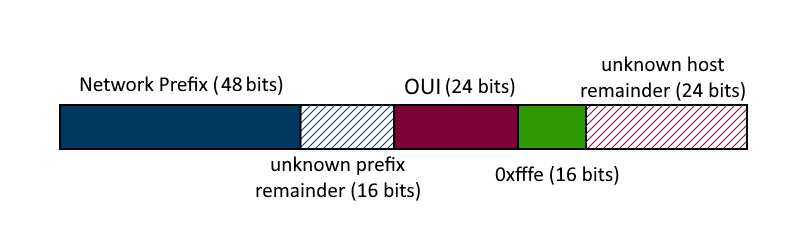
\includegraphics[totalheight=8cm]{ipv6addr.png}
    \caption{Example of the remaining search space when scanning /48 IPv6 prefix advertisements for devices with SLAAC-assigned addresses.}
    \label{ipv6addr}
\end{figure}

Fully-formed 64-bit IPv6 address prefixes can also be obtained through side-channel attacks, such as harvesting addresses from responses to phishing emails, or eavesdropping on network traffic.
These are important security risks to consider, particularly because attacks using these approaches are less complex to perform than using BGP data as described in this section.
For obvious ethical reasons, in-depth analysis of these side-channel attacks are beyond the scope of this project, but proposed fixes to improve IPv6 security could still help to mitigate any potential damage they may cause;
improvements in IPv6 addressing security provides additional protection no matter the method of attack.

\subsection{Relevance of Work to Recent Events}
The threat posed by mass recruitment of poorly secured IoT devices is not theoretical.
Malware families like Mirai, IoT Reaper, and Mozi have taken advantage of lax IoT security in recent years to recruit hosts for botnets, with Mirai in particular amassing enough bots to generate over 1Tb/s of traffic used for distributed denial of service (DDoS) attacks \cite{mirai-traffic}.
When working as intended, Mirai denial of service attacks managed to take down Dyn, a popular DNS provider, which prevented many users from accessing popular sites like Amazon and Twitter.
When not working as intended, Mirai still managed to cause a widespread service outage for TalkTalk and Deutche Telekom customers by taking 900,000 infected routers offline;
this was caused by a buggy implementation of Mirai which unintentionally deactivated routers instead of using them to contribute to DDoS attacks \cite{antonakakis2017}.

As shown by the notable increase in the number of IPv6 prefix advertisements in the 2020 BGP dataset compared to the 2014 equivalent, IPv6 deployment is on the rise.
The number of IoT devices on the market is also increasing, with devices like Amazon Alexa being specifically marketed for domestic use by users who are unlikely to know how to secure their home networks.
There is a persistent myth that IPv6 is more resilient against scanning attacks (and therefore mass host recruitment) because the address space is too large to search exhaustively;
the aim of this work is to disprove this, and to emphasise that security through obscurity is not a reliable defense strategy when working with IPv6.
This is particularly true of IoT device manufacturers, who are infamous for treating security as an afterthought instead of a primary consideration.
Mass manufacture of devices which are vulnerable to these attacks is unethical, particularly when they are marketed at `non-technical' users as a quality-of-life improvement or when they are used for sensitive data, such as domestic video capture;
warning manufacturers about the risks of these attacks and advising on how to prevent them is important.

%==================================================================================================
\section{Thesis Statement}

IPv6 addressing is said to be resistant to scanning attacks due to exhaustive searches not being possible in a 128-bit space.
This is partially true:
exhaustive searches are not possible, but the search space can be reduced to feasible ranges through the use of publicly accessible data, such as BGP advertisements and organisationally unique identifiers.
I will prove this by demonstrating that scanning an address space for specific classes of devices is possible, and will identify how these scanning attacks can be prevented, particularly for IoT devices which are liable to use outdated IPv6 addressing techniques.


%0=================================================================================================
\section{Research Plan}

Table \ref{research-timeline} gives the proposed timeline for each of the experiments described below.

\begin{table}[]
\centering
\label{research-timeline}
\begin{center}
	\begin{tabular}{|l|l|l|}
		\hline
		Experiment & Duration & Completion Date   \\ \hline
		Privacy addresses and SLAAC addresses & 2 weeks & July 2020   \\ \hline
		IoT IPv6 usage & 2 months & September 2020     \\ \hline
		Find IoT devices on local networks & 3 months & January 2021  \\ \hline
		IPv6 prefix length & 9 months & September 2021  \\ \hline
		Current use of IPv6 in malware & 3 months & January 2022
		Offered services  & 9 months & September 2022  \\ \hline
		Security improvements & 7 months & April 2023  \\ \hline
		Thesis write-up & 6 months & October 2023 
		\hline
	\end{tabular}
	\caption{Anticipated timeline of future experiments}
\end{center}
\end{table}

\subsection{Determine if privacy addresses replace SLAAC addresses}
In order to determine whether more complex devices like smartphones, laptops, and desktops are at risk of being located over IPv6 using their MAC address information alongside IoT devices, I need to find out whether SLAAC addresses are assigned in addition to privacy addresses, or whether they replace them.
An initial starting point would be to search documentation on MSDN, Linux kernel code, BSD kernel code, and Apple developer documentation to find out if IPv6 SLAAC addresses remain active even when a privacy address has been assigned.
I can then attempt to contact machines using various mainstream operating systems using local scanning knowledge to find out if any response is given to contact with SLAAC address, and note whether these outcomes match what is described in the documentation or what should be expected from the source code.
Local scans will also be performed in an attempt to locate virtual machines, to see if the virtual machine addressing conventions outlined in RFC7707 \cite{rfc-ipv6-rec} are used in practice.

\subsection{Determine how many IoT devices actually use IPv6}
IoT devices are infamous for being insecure;
however, in order to know whether they can be mass recruited by attackers using IPv6 scans, it is important to know how many of these devices actually use IPv6 in the first place.
Imperial College London and Northeastern University both have labs with a wide range of IoT devices.
If either of these institutions are willing to allow me to access these labs, I can obtain and parse network logs to see how many devices are communicating using an IPv6 address.
From these, it should be possible to identify whether specific manufacturers consistently use IPv6 for their devices, and whether they use privacy extensions with robust random number generation.

\subsection{Find specific devices in a local network}
Using the local scanning heuristics proposed in section \ref{current-work-local}, I will attempt to locate specific types of IoT device which were found on this network previously by their IPv6 address.
If virtual machines and devices like smartphones, laptops, and desktops are found to be reachable through their SLAAC addresses, this experiment can be repeated for these devices as well.


\subsection{Longer term study of advertised IPv6 prefix length}
Finding devices with Internet-wide IPv6 scans is unethical, so research into these scans needs to be mostly theoretical.
It might be possible to try locating a device a device I own across the Internet from another network, but no substantial datasets can be gathered.
Identifying longer-term trends in advertised IPv6 prefixes means that we can see how much the scanning space can be reduced by in specific use-cases;
several ISPs serving home environments advertise /56 prefixes, which would be more appealing to attackers looking to recruit, for example, smart TVs, while attackers looking to recruit hosts for malware leasing in an enterprise network may want to scan a different range of prefixes more commonly associated with that kind of environment.

\subsection{Investigate current use of IPv6 in malware}
Several malware variants, such as ZeuS, a banking trojan, are known to use IPv6 for peer-to-peer traffic and tunneling \cite{zeus}.
Others use IPv6 unknowingly as a result of being composed of recycled malicious code from other samples.
To the best of my knowledge, none are known to use IPv6 scanning for host recruitment as yet, but this may change within the next three years.
If any novel samples are found to use IPv6 scanning during the course of this PhD, I will perform analysis of the sample (binary, dynamic linked library, etc.) to identify exactly how it performs these scans, and whether they matched predictions made about scanning strategies earlier in the PhD.

Surveying the use of IPv6 within current malware samples would allow me to determine how much use malware authors currently have for IPv6, and to get an idea of how much expertise is involved in writing IPv6-enabled malware.
Collaboration with anti-virus companies would be very beneficial here;
access to large repositories of catalogued samples, awareness of this work within industry, and the opportunity to learn from expert analysis would be an excellent opportunity.

\subsection{Identify which kinds of services are offered by cybercrime organisations}
IoT botnet operations for DDoS attacks are no longer a viable business venture since Mirai was released as open source malware for this purpose \cite{mirai-open-source}.
Malware-as-a-service operations currently use trojans, like Emotet and the potentially defunct Dreambot, as loader software on smartphones, laptops, and desktops, which are leased to ransomware gangs \cite{emotet-lease} \cite{dreambot}.
This is a fast-moving environment, so it's possible that IoT device recruitment for non-DDoS purposes could be happening by this point.

There are recent signs of malware-as-a-service cartels co-operating with each other to a much greater degree than usual, under the banner of Maze ransomware \cite{maze-ransomware}.
This could change the threat landscape significantly, and is worth investigating as part of this PhD;
more organised collaboration could further increase the complexity of the malware these organisations are about to produce, and could potentially allow for recruitment via complex IPv6 scans to occur in the wild.

\subsection{Security improvements}
Proving the viability of IPv6-based attacks and their potential use-cases is important, but responsibility also needs to be taken for suggesting which measures would have stopped these attacks from succeeding;
finding ways to block these scans is important to improve security for any Internet-connected environment, whether that's a large enterprise network, or a home network served by a default ISP-supplied router.
Insecure IoT devices will have the most obvious IPv6 security flaws to fix, but developers of operating systems for smartphones, laptops, and desktops may also have areas to fix.
Security advice could be given in the form of amendments to existing IETF RFCs related to IPv6, or specific recommendations to IoT device manufacturers.

\subsection{Thesis write-up}
The experiments listed above will hopefully have resulted in one or more publications each, and will have been written up as a chapter of the thesis.
The last few months of the PhD will be spent writing up final conclusions, and ensuring that the thesis flows well as a single document.


%==================================================================================================
% Set the bibliography style. Choose one of the following, depending on the
% document class being used:
%
%   \bibliographystyle{abbrv}                 When using article class
%   \bibliographystyle{IEEEtran}              When using IEEE style
%   \bibliographystyle{ACM-Reference-Format}  When using ACM style

\bibliographystyle{ACM-Reference-Format}

% Load the bibliography file(s) for this paper:
\bibliography{example}

%==================================================================================================
% The following information gets written into the PDF file information:
\ifpdf
  \pdfinfo{
    /Title        (...)
    /Author       (...)
    /Subject      (...)
    /Keywords     (..., ..., ...)
    /CreationDate (D:20150827110616Z)
    /ModDate      (D:20150827110616Z)
    /Creator      (LaTeX)
    /Producer     (pdfTeX)
  }
  % Suppress unnecessary metadata, to ensure the PDF generated by pdflatex is
  % identical each time it is built. This needs pdfTeX 3.14159265-2.6-1.40.17
  % or later.
  \ifdefined\pdftrailerid
    \pdftrailerid{}
    \pdfsuppressptexinfo=15
  \fi
\fi
%==================================================================================================
\end{document}
% vim: set ts=2 sw=2 tw=75 et ai:
